\subsection{原理}
\begin{align*}
    &H_1 = \Sigma_{XX}^{-1} \Sigma_{XXY} \Sigma_{XX}^{-1} \\
    &span(H_1) \subseteq S_{Y|X}
\end{align*}
\subsection{样本计算流程}
\begin{enumerate}
    \item 将$X_1,\dots,X_n$标准化为$Z_1,\dots,Z_n$
    \item 计算$\hat{\Sigma}_{ZZY}E_n(ZZ^TY),\quad \hat{\Sigma}_{XX}Var_n(X)$
    \item 计算$\hat{\Sigma}_{ZZY}$的前$q$个特征向量$u_1,\dots,u_n$,则对$S_{Y|X}$中向量的估计为$v_k=\hat{\Sigma}_{XX}^{-1/2}u_k,k=1,\dots,q$
\end{enumerate}


\subsection{线性回归}
设定样本量为1000,样本$X$维度为$5$,降维后维度为$2$.一次的计算结果$H_1,H_2$如下表所示

\begin{table}[htbp]
\centering
\caption{线性回归结果}
\label{tab:norm}
\begin{tabular}{l|l|ll}
\hline
\multicolumn{2}{c|}{$H_1$} & \multicolumn{2}{c}{$H_2$}                    \\ \hline
-0.7193995  & 0.07794245   & \multicolumn{1}{l|}{0.6920215}  & 0.4112301  \\ \hline
-0.2187786  & -0.24974545  & \multicolumn{1}{l|}{-0.1080706} & -0.7261988 \\ \hline
-0.5618548  & 0.28103448   & \multicolumn{1}{l|}{0.6192357}  & -0.3741050 \\ \hline
-0.1909770  & -0.92664516  & \multicolumn{1}{l|}{-0.2790291} & 0.2171582  \\ \hline
-0.3313467  & -0.03092594  & \multicolumn{1}{l|}{-0.2530621} & 0.2974159  \\ \hline
\end{tabular}
\end{table}

接下来判断维度的增大对降维效果的影响,设定$X$维度依次为$3-20$,统一降维至二维,判断依据为两个空间的距离.如下图所示
\begin{figure}[htbp]
    \centering
    \includegraphics[width=0.8\textwidth]{image/norm.eps}
    \caption{线性回归下维度对降维效果的影响}
\end{figure}


\subsection{泊松回归}
\begin{figure}[htbp]
    \centering
    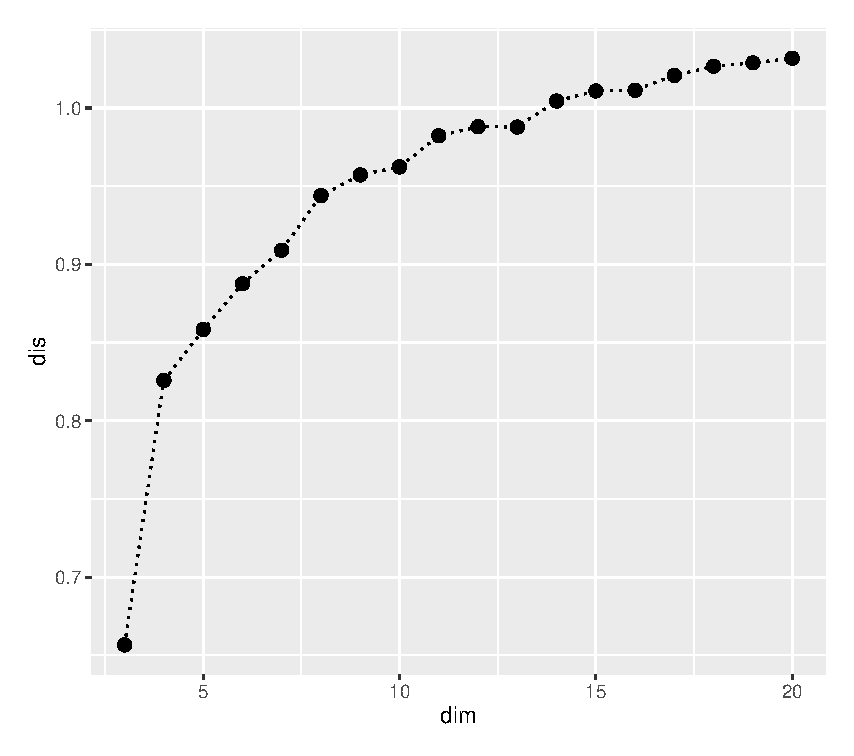
\includegraphics[width=0.8\textwidth]{image/pois_phd.eps}
    \caption{泊松回归下维度对降维效果的影响}
\end{figure}

\subsection{Logistic回归}

\begin{figure}[htbp]
    \centering
    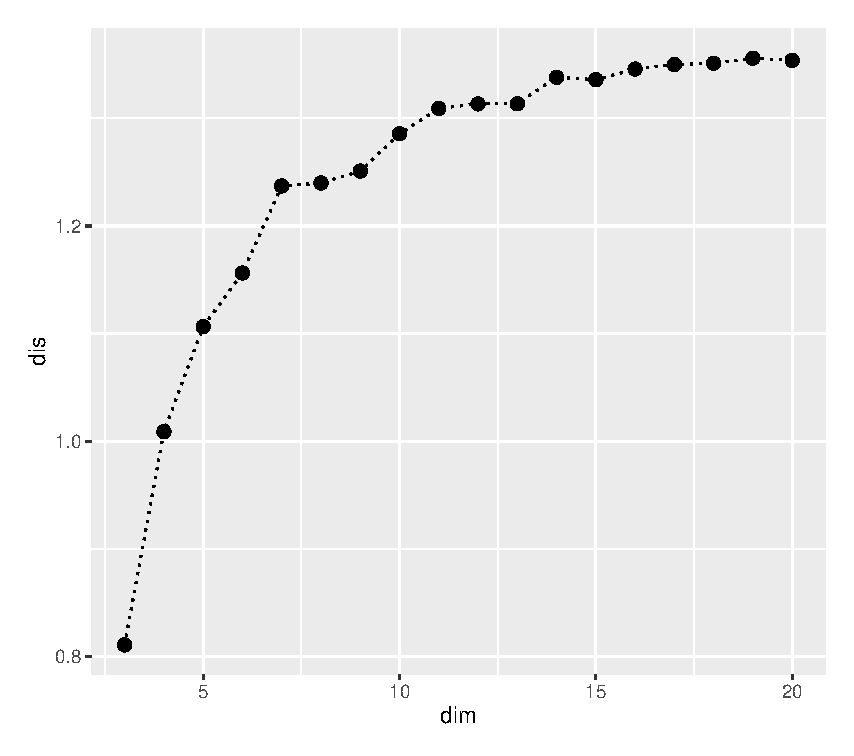
\includegraphics[width=0.8\textwidth]{image/logit_phd.eps}
    \caption{logistics回归下维度对降维效果的影响}
\end{figure}

\subsection{生成cos函数关系}
\begin{figure}
    \centering
    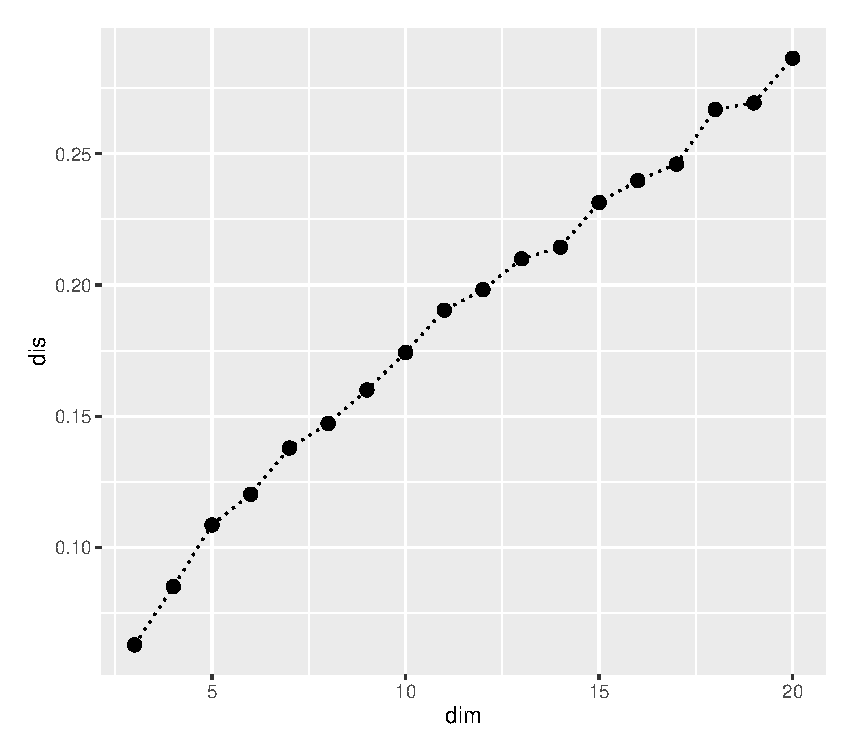
\includegraphics[width=0.8\textwidth]{image/cos_phd.eps}
    \caption{cos函数生成的数据下维度对降维效果的影响}
\end{figure}


